\documentclass[10pt,a4paper,final]{article}
\usepackage[utf8]{inputenc}
\usepackage[portuguese]{babel}
\usepackage[T1]{fontenc}
\usepackage[margin=1in]{geometry}
\usepackage{amsmath}
\usepackage{amsfonts}
\usepackage[table]{xcolor}
\usepackage{graphicx}
\usepackage{multirow}
\usepackage{setspace}
\usepackage{amssymb}
\usepackage{lscape}
\usepackage{plano}
%\usepackage[alf]{abntex2cite}
\usepackage{natbib}

\programa{Engenharia Elétrica}
\area{Engenharia de Computação}
\aluno{Jefferson Caros de Mendonça}
\orientador{Edson Satoshi Gomi}
\curso{Mestrado}
\dataIngresso{14/09/2016}
\titulo{Modelo para Mineração de Dados -
Análise das Perguntas e Respostas do Site Stack Overflow}
\resumo{
As transformações no cenário tecnológico provocam mudanças constantes que exigem atualização contínua. Como fonte de estudos e atualização, profissionais da área de computação diariamente recorrem à diversas fontes de informação, dentre elas destaca-se o site StackOverflow, maior comunidade de perguntas e respostas onde os usuários podem aprender, trocar experiências e compartilhar conhecimento.
O objeto deste projeto de pesquisa é propor um modelo de mineração de dados que consiga catalogar as perguntas desta comunidade, facilitando a busca por informações e detecção dos principais questionamentos discutidos .}

\palavrachave{information retrieval}
\palavrachave{text mining}
\palavrachave{text classification}
\palavrachave{automated text categorization}
\palavrachave{keyword extraction}
\palavrachave{document indexing}
\palavrachave{StackOverflow}


\begin{document}

    \folhaDeRosto

    \plano
    
    \section{Introdução}
    
    Não raro a evolução na área computacional se desenvolve em ritmo acelerado, novos algoritmos, técnicas para processamento de imagem, computação distribuída, \emph{linguagens de programação} aprimoram suas API's constantemente, construindo e desconstruindo métodos e muitas vezes incorporam novos paradigmas. Essas transformações no cenário tecnológico provocam mudanças constantes exigindo atualização contínua.
	Para dar vazão a este dinamismo, profissionais da área de computação diariamente recorrem a cursos presenciais, a distância, livros, revistas e claro \textit{websites}. Dentre estas mídias, merece destaque o fórum \textit{Stack Overflow}, maior comunidade \textit{online} de perguntas e respostas onde os usuários podem aprender, trocar experiências e compartilhar conhecimento.
    
    \subsection{Contextualização do Problema}
    O número de questões em sites de perguntas e respostas crescem diariamente, faz-se necessário categorizar os assuntos discutidos em tópicos, para uma busca mais fácil e dinâmica.  \cite{Yasotha2016} observam que a categorização manual de textos, pode ser feita somente por especialistas e requer muito tempo. Como consequência é de grande importância a categorização e classificação de documentos de forma automática.

    \subsection{Objetivos}
Propor um modelo de mineração de dados sobre a comunidade online de perguntas e respostas StackOverflow, onde seja possível categorizar de forma automática os tópicos mais relevantes discutidos.

    \subsection{Justificativas}

O método proposto por \cite{Arash2016} categorizou os dados do StackOverflow. Em seu projeto os autores classificaram os assuntos utilizando as tags da própria pergunta, e então utilizaram o site Wikipédia para validar o tópico encontrado e identificar a qual categoria ele pertence. A proposta desta pesquisa, é prover a categorização e classificação de textos que faça apenas uso do texto disponível nas perguntas e respostas, não utilizando recursos adicionais como tags que fornecem dica sobre qual é o tópico de um assunto específico.

   \subsection{Organização do texto}

Para melhor definir qual o posicionamento do presento projeto, no capítulo seguinte será detalhado em maior profundidade os projetos que abordaram a categorização de documentos, inclusive àqueles que também fizeram uso do site StackOverflow como base de dados. Então a proposta será detalhada quantos aos procedimentos para a indexação das perguntas e respostas, desde a seleção do conteúdo original, armazenamento em banco de dados e extração e por fim serão exibidos os resultados esperados.

 \section{Revisão da Literatura}
   


   \section{Detalhamento da Proposta}



%%\begin{figure}[!htb] 
%%\centering
%%    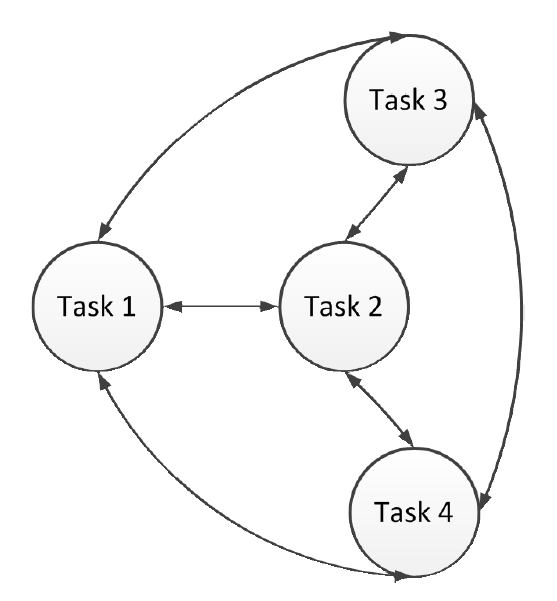
\includegraphics[height=5cm]{Figures/PTL}\label{fig:PTL}   
%% \caption{Fluxo de conhecimento na T L com transferência paralela (PTL).}
%%\end{figure}

  
    \section{Plano de Trabalho}



    \subsection{Resultados Desejados e Validação}
    
A análise será feita sobre os mesmo dados da pesquisa realizada por \cite{Arash2016}, os resultados obtidos anteriormente serão a base para a medição da acurácia da nova proposta e então será possível aplicar o modelo desenvolvido sem a utilização de tags pré-definidas, possibilitando a construção de catálogos para outros sites de perguntas e respostas.
 
    \subsection{Atividades e Cronograma}
    
Atividades e Cronograma.

\nocite{Joorabchi2015}
\nocite{Manning2009}
\nocite{Mihalcea2007}
\nocite{Mihalcea2001}
\nocite{Mihalcea2004}
\nocite{Miotto2013}
\nocite{Posch2014}
\nocite{Roul2015}
\nocite{Udell2005}
\bibliographystyle{apalike}
\bibliography{Refs}{}  


    

\end{document}
    